\documentclass[11pt]{article}
\pagestyle{empty}
%\usepackage[latin1]{inputenc}
\usepackage[utf8]{inputenc}
\usepackage{a4wide}
\usepackage{amsmath}
\usepackage{amssymb}
\usepackage{amsthm}
\usepackage{german}
\usepackage{multirow,array}
\usepackage{hyperref}
 \usepackage{graphicx}
%\usepackage{ipe}
%\input{thmstyle-ger}

\parindent0mm
\sloppy

% Basic data
\newcommand{\VORLESUNG}{Induktive Statistik für Soziologinnen und Soziologen}
\newcommand{\STAFF}{Mariana Nold}
\newcommand{\ASSIGNMENT}{2}
\newcommand{\HANDOUT}{Montag, den 13. November   2017}
\newcommand{\DELIVER}{keine Abgabe, wird in der Übung besprochen}
\newcommand{\PRACTICAL}[1]{\marginpar{\tiny {\bf Aufgabe \\ abgeben!} #1}}
\newcommand{\FAUFTRAG}[1]{\marginpar{\tiny {\bf selbst entdeckendes Verstehen} #1}}
\newcommand{\titel}{Grundlagen des statistischen Testens}
\newcommand{\startwert}{3}

% Arbitrary packages and settings

\newcommand{\N}{\mathbb{N}}
\newcommand{\floor}[1]{\lfloor{#1}\rfloor}
\newcommand{\ceil}[1]{\lceil{#1}\rceil}
\newcommand{\half}[1]{\frac{#1}{2}}
\newcommand{\punkte}[1]{{\small{ }(#1 Punkte)}}
\newcommand{\punkt}[1]{{\small{ }(#1 Punkt)}}

\newcommand{\aufgabe}[1]{\item{\bf #1}}
\newcommand{\hinweis}{{\em Hinweis}}

\begin{document}
% Document title

\begin{center}
\ASSIGNMENT{}. Übungsblatt vom \HANDOUT{} zur Vorlesung 
\vspace*{0.5cm}

{\Large \VORLESUNG{}}
%\PRACTICAL{}
(\STAFF{}) 


\vspace*{0.5cm}
{\textbf{Thema:} \titel{}\\}
\vspace*{0.2cm}

{\small Abgabe: \DELIVER{}}
\vspace*{1cm}
\end{center}

Wichtige Definitionen:
\begin{enumerate}
\item{Inferenzschluss}
\item{gerichtete Hypothese}
\item{ungerichtete Hypothese}
\item{Fehler 1. Art ($\alpha$-Fehler)}
\item{Fehler 2. Art ($\beta$-Fehler)}
\item{Teststatistik des Zwei-Stichproben t-Test}
\item{Ablauf des Zwei-Stichproben t-Test}
\item{kritischer Wert und Ablehnbereich}
\item{p-Wert}
%\item{Binäre Variable und  Bernoulliverteilung}
%\item{Binomialverteilung}
\end{enumerate}
\vspace{2cm}
\begin{enumerate}\addtocounter{enumi}{\startwert}


Nutzen Sie die sechsseitige Übersicht über wichtige statistische Tests und Grundprinzipien von Hypothekentests. Diese Übersicht dürfen Sie auch in der
Klausur verwenden.


%\aufgabe{Aufgabe}
%\aufgabe{Der $\chi^{2}$-Test:  Statusverlustangst und relative Deprivation im Thüringen-Monitor $2015$}\\
%(vgl. Aufgabe 18, des 5. Übungsblattes im letzten Semester.)\\
%Leseempfehlung: LWLG: S. 212-218\\
%\vspace{0.5cm}
% Augabe mit der Notation von LM lösen und die äquivalente Notation angeben
Zur Erinnerung an Definitionen aus  der Vorlesung:

Die Frage nach der Statusverlustangst: ``Es macht mir Sorgen, durch die gesellschaftliche Entwicklung immer mehr auf die Verliererseite
 des Lebens zu geraten.''
 \begin{itemize}
   \item {Die Antwortkategorien: ``lehne ab,'' ``stimme zu''}
    \item {Im Datensatz: ``lehne ab = nein,'' ``stimme zu = ja''}
  \end{itemize} 
  Die Frage zur Deprivation: ``Im Vergleich dazu, wie andere hier in Deutschland leben: 
   Glauben Sie, dass Sie Ihren gerechten Anteil erhalten, 
   mehr als Ihren gerechten Anteil, etwas weniger oder sehr viel weniger?''
   \begin{itemize} 
   \item{Die Antwortkategorien: ``erhalte sehr viel weniger,'' ``erhalte etwas weniger,''  ``erhalte gerechten Anteil,''         
  ``erhalte mehr als gerechten Anteil,''  ``weiß nicht,'' ``keine Angabe''}
  \item{Im Datensatz:
    \begin{description}
    
     \item {
       \[
     \text{``erhalte weniger''}=\left\{\begin{array}{ll} \text{``erhalte sehr viel weniger,''} \\
         \text{``erhalte etwas weniger''}\end{array}\right. 
  \]
     }
      \item {
       \[
     \text{``erhalte genug''}=\left\{\begin{array}{ll} \text{``erhalte gerechten Anteil,''} \\
         \text{``erhalte mehr als gerechten Anteil''}\end{array}\right. 
  \]
     }
     %\item {(``erhalte gerechten Anteil,'' ``erhalte mehr als gerechten Anteil'')= ``erhalte genug,''}
    
    \end{description}
      }
 \end{itemize}

Im Thüringen-Monitor 2015 haben $940$ Personen sowohl die Frage nach der 
Statusverlustangst als auch nach der Deprivation beantwortet. Die anderen $70$ Personen haben mit ``weiß nicht'' oder ``keine Angabe''
geantwortet oder die Antwort vollständig verweigert. Die  Vierfeldertafel \ref{depri_angst} zeigt die bivariaten Häufigkeiten
der $940$ Personen.

%        erhalte.weniger erhalte.genug
%   nein             289           362
%   ja               214            75

  \begin{table}[ht]
\centering
\caption{Bivariate Häufigkeit: Statusverlustangst $Y$ und Deprivation $X$}



\begin{center}
\begin{tabular}{|c|c|c|}
	\hline %   
             & erhalte weniger   & erhalte genug  \\ \hline
        nein & $289$  & $362$                  \\ \hline
          ja & $214$  & $75$        \\ \hline
\end{tabular}
\end{center}
\label{depri_angst}
\end{table}
Lösen Sie die folgenden Aufgaben mit Hilfe von  \texttt{STATA 14:}
\begin{enumerate}
 \item {Lesen Sie mit dem Befehl \texttt{. use ``monitor\_15.dta'', clear} den Datensatz ein und erstellen  Sie die Vierfeldertafel \ref{depri_angst}.}
 \item{Geben Sie den Befehlt \texttt{. tab2 Angst Deprivation, chi2} in das Command-Window ein
 und erklären lesen Sie den Werte des $\chi^{2}$-Koeffizienten und das  ab.}
 \item{Schlagen Sie die Formelsammlung auf S 6 auf. Geben Sie die Definition des $\chi^{2}$-Koeffizienten an und erklären Sie warum hohe Werte gegen eine Unabhängigkeit der beiden
 Merkmale $X$ und $Y$ sprechen.}
 \item{Erklären sie mit Bezug auf die angegeben $2 \times 2$ Kreuztabelle, was man unter einem Inferenzschluss versteht. }
 \item{Wir möchten nachweisen, dass die beiden Merkmale $X$ und $Y$ (stochastisch) abhängig sind, wie können entsprechend die Nullhypothese
 und die Forschungshypothese formuliert werden?}% FT S. 466
 \item{Was versteht man unter dem Signifikanzniveau bzw. der Irrtumswahrscheinlichkeit?}
 \item{Legen Sie das Signifikanzniveau fest und suchen Sie im \texttt{STATA-output} des Befehls \texttt{. tab2 Angst Deprivation, chi2}
 nach dem p-Wert. Kann die Forschungshypothese nachgewiesen werden?}
 \item{Es lässt sich zeigen, dass der $\chi^{2}$-Koeffizient unter $H_{0}$ einer $\chi^{2}$-Verteilung mit einem Freiheitsgrad folgt. Diese ist in Abbildung
 \ref{abb1} dargestellt. Es ist auch der kritische Wert $k$ eingezeichnet. Der kritische Wert ist $3.84.$
 \begin{itemize}
 \item[i)]{Der  $\chi^{2}$-Koeffizient entspricht im  $\chi^{2}$-Test der Teststatistik. Vergleichen Sie den Wert der Teststatistik mit dem kritischen Wert 
 $k=3.84.$ }
 \item[ii)]{Markieren Sie den Ablehnbereich farbig und malen Sie die Fläche zwischen  Ablehnbereich und Dichtkurve aus. Wie hoch ist der Anteil der
 ausgemalten Fläche an der Fläche unter der Dichterkurve. }
 \item[iii)]{Quantifizieren Sie die Unsicherheit des Inferenzschlusses indem Sie Auskunft über den $\alpha$- und $\beta$-Fehler geben.}
 \end{itemize}
 }
\end{enumerate}
 \begin{figure}[ht]
 	\centering
 	      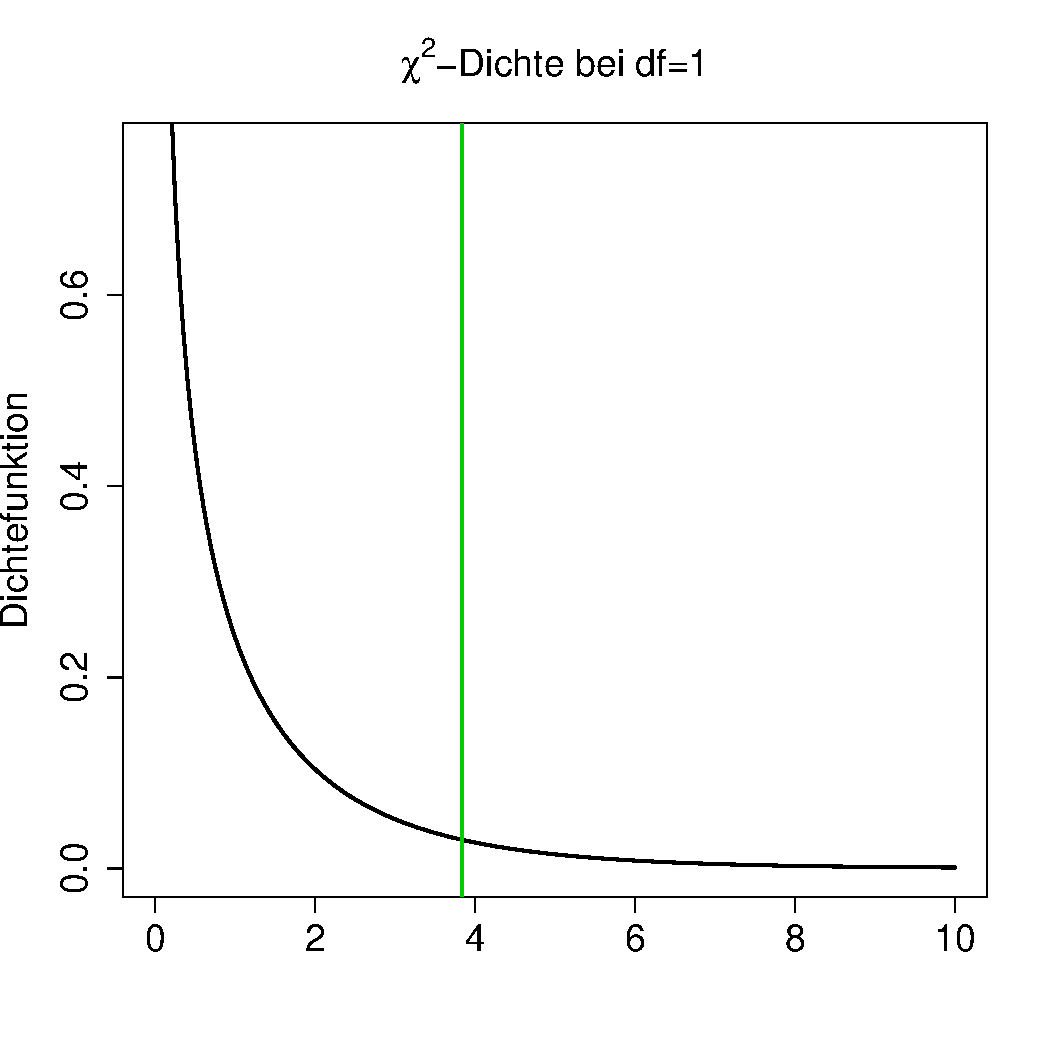
\includegraphics[width=0.85\textwidth]{chi2.pdf}
 	      \caption{Dichte der $\chi^{2}$-Verteilung mit einem Freiheitsgrad
 	       \label{abb1}}
 	\end{figure}
% https://stats.idre.ucla.edu/other/mult-pkg/whatstat/ 	
%http://www.reed.edu/psychology/stata/analyses/nonparametric/bitest.html
\aufgabe{Approximativer Binomialtest}

Ein Politiker behauptet in einer Pressemitteilung mit Bezug auf den Thüringen-Monitor $2015,$ dass der Anteil der Thüringer Wahlbevölkerung
der angibt weniger als seinen Gerechten Anteil zu erhalten mittlerweile auf über $50\%$ gestiegen ist. Im Klartext mindestens eine von zwei
Personen über 18 Jahre ist der Meinung benachteiligt zu sein. Schlagen Sie die Formaltsammlung auf S. 3 auf, um diese Aufgabe zu bearbeiten.

% Überblick über die Tests
%http://statistik-dresden.de/archives/6026
%http://www.statistics4u.info/fundstat_germ/ee_baum_2_3_1.html
% Überblick: STATA
% https://stats.idre.ucla.edu/other/mult-pkg/whatstat/
\begin{enumerate}
\item{Formulieren Sie passend zu der Behauptung des Politkerns die Forschungshypothese und die Nullhypothese. Handelt es sich um eine gereichtet 
oder eine ungerichtet Hypothese?}
\item{}
\item{}
\item{}
\item{}
\item{}
\end{enumerate}
% https://www.beratung-statistik.de/statistik-beratung-infos/stata-tutorial/regression-stata-interpretation/
%https://www.stata.com/statalist/archive/2008-06/msg00018.html
%https://www.beratung-statistik.de/statistik-beratung-infos/stata-tutorial/stata-nachhilfe-zufallszahlen/
\newpage
\aufgabe{Ein Intervall, dass alle Nullhypothesen enthält, die nicht abgelehnt werden} % Müssen Sie selber machen
% Mit Bezug zu der Aufgabe davor: Was kann er behaupten?
\begin{enumerate}
\item{}
\item{}
\item{}
\item{}
\end{enumerate}

\end{enumerate}
\end{document}
